\section{Spark::Sp\-Resource\-Path Class Reference}
\label{classSpark_1_1SpResourcePath}\index{Spark::SpResourcePath@{Spark::SpResourcePath}}
{\tt \#include $<$Sp\-Resource\-Path.h$>$}

Collaboration diagram for Spark::Sp\-Resource\-Path:\begin{figure}[H]
\begin{center}
\leavevmode
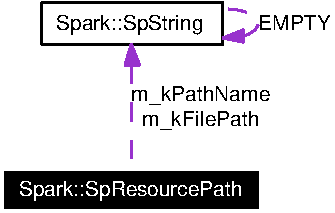
\includegraphics[width=98pt]{classSpark_1_1SpResourcePath__coll__graph}
\end{center}
\end{figure}


\subsection{Detailed Description}
Resource utility class for querying a file system and loading datafiles. 

Definition at line 41 of file Sp\-Resource\-Path.h.\subsection*{Public Types}
\begin{CompactItemize}
\item 
typedef stat {\bf File\-Stat}
\begin{CompactList}\small\item\em Type Definitions:. \item\end{CompactList}\end{CompactItemize}
\subsection*{Public Member Functions}
\begin{CompactItemize}
\item 
{\bf Sp\-String} \& {\bf filepath} ()
\begin{CompactList}\small\item\em Access Methods:. \item\end{CompactList}\item 
const {\bf Sp\-String} \& {\bf filepath} () const
\item 
{\bf Sp\-String} \& {\bf pathname} ()
\item 
const {\bf Sp\-String} \& {\bf pathname} () const
\item 
{\bf Sp\-String\-Array} \& {\bf searchpath} ()
\item 
const {\bf Sp\-String\-Array} \& {\bf searchpath} () const
\item 
void {\bf add\-Path} (const {\bf Sp\-String} \&rk\-Pathname)
\begin{CompactList}\small\item\em Attributes:. \item\end{CompactList}\item 
{\bf Sp\-String} {\bf get\-Path} (const {\bf Sp\-String} \&rk\-Filename)
\item 
{\bf Sp\-String} {\bf get\-File} (const {\bf Sp\-String} \&rk\-Filename)
\item 
char $\ast$ {\bf load\-Text\-File} (const char $\ast$ac\-Filename)
\begin{CompactList}\small\item\em File Methods:. \item\end{CompactList}\item 
{\bf Sp\-String} {\bf load\-Text\-File} (const {\bf Sp\-String} \&rk\-Filename)
\item 
FILE $\ast$ {\bf load\-Data\-File} (const {\bf Sp\-String} \&rk\-Filename, const char $\ast$ac\-Mode=\char`\"{}rb\char`\"{})
\item 
int {\bf get\-File\-Stats} (const {\bf Sp\-String} \&rk\-Filename, {\bf File\-Stat} $\ast$pk\-Stat)
\end{CompactItemize}


\subsection{Member Typedef Documentation}
\index{Spark::SpResourcePath@{Spark::Sp\-Resource\-Path}!FileStat@{FileStat}}
\index{FileStat@{FileStat}!Spark::SpResourcePath@{Spark::Sp\-Resource\-Path}}
\subsubsection{\setlength{\rightskip}{0pt plus 5cm}typedef struct stat {\bf Spark::Sp\-Resource\-Path::File\-Stat}}\label{classSpark_1_1SpResourcePath_w0}


Type Definitions:. 

Definition at line 50 of file Sp\-Resource\-Path.h.

Referenced by get\-File\-Stats(), and load\-Text\-File().

\subsection{Member Function Documentation}
\index{Spark::SpResourcePath@{Spark::Sp\-Resource\-Path}!addPath@{addPath}}
\index{addPath@{addPath}!Spark::SpResourcePath@{Spark::Sp\-Resource\-Path}}
\subsubsection{\setlength{\rightskip}{0pt plus 5cm}void Spark::Sp\-Resource\-Path::add\-Path (const {\bf Sp\-String} \& {\em rk\-Pathname})\hspace{0.3cm}{\tt  [inline]}}\label{classSpark_1_1SpResourcePath_a6}


Attributes:. 

Definition at line 77 of file Sp\-Resource\-Path.h.\index{Spark::SpResourcePath@{Spark::Sp\-Resource\-Path}!filepath@{filepath}}
\index{filepath@{filepath}!Spark::SpResourcePath@{Spark::Sp\-Resource\-Path}}
\subsubsection{\setlength{\rightskip}{0pt plus 5cm}const {\bf Sp\-String}\& Spark::Sp\-Resource\-Path::filepath () const\hspace{0.3cm}{\tt  [inline]}}\label{classSpark_1_1SpResourcePath_a1}


Definition at line 59 of file Sp\-Resource\-Path.h.\index{Spark::SpResourcePath@{Spark::Sp\-Resource\-Path}!filepath@{filepath}}
\index{filepath@{filepath}!Spark::SpResourcePath@{Spark::Sp\-Resource\-Path}}
\subsubsection{\setlength{\rightskip}{0pt plus 5cm}{\bf Sp\-String}\& Spark::Sp\-Resource\-Path::filepath ()\hspace{0.3cm}{\tt  [inline]}}\label{classSpark_1_1SpResourcePath_a0}


Access Methods:. 

Definition at line 56 of file Sp\-Resource\-Path.h.\index{Spark::SpResourcePath@{Spark::Sp\-Resource\-Path}!getFile@{getFile}}
\index{getFile@{getFile}!Spark::SpResourcePath@{Spark::Sp\-Resource\-Path}}
\subsubsection{\setlength{\rightskip}{0pt plus 5cm}{\bf Sp\-String} Sp\-Resource\-Path::get\-File (const {\bf Sp\-String} \& {\em rk\-Filename})}\label{classSpark_1_1SpResourcePath_a8}


Definition at line 86 of file Sp\-Resource\-Path.cpp.

References Spark::Sp\-String::Size\-Type.\index{Spark::SpResourcePath@{Spark::Sp\-Resource\-Path}!getFileStats@{getFileStats}}
\index{getFileStats@{getFileStats}!Spark::SpResourcePath@{Spark::Sp\-Resource\-Path}}
\subsubsection{\setlength{\rightskip}{0pt plus 5cm}int Sp\-Resource\-Path::get\-File\-Stats (const {\bf Sp\-String} \& {\em rk\-Filename}, {\bf File\-Stat} $\ast$ {\em pk\-Stat})}\label{classSpark_1_1SpResourcePath_a12}


Definition at line 208 of file Sp\-Resource\-Path.cpp.

References File\-Stat.

Referenced by load\-Text\-File().\index{Spark::SpResourcePath@{Spark::Sp\-Resource\-Path}!getPath@{getPath}}
\index{getPath@{getPath}!Spark::SpResourcePath@{Spark::Sp\-Resource\-Path}}
\subsubsection{\setlength{\rightskip}{0pt plus 5cm}{\bf Sp\-String} Sp\-Resource\-Path::get\-Path (const {\bf Sp\-String} \& {\em rk\-Filename})}\label{classSpark_1_1SpResourcePath_a7}


Definition at line 16 of file Sp\-Resource\-Path.cpp.

References Spark::Sp\-String::Size\-Type.\index{Spark::SpResourcePath@{Spark::Sp\-Resource\-Path}!loadDataFile@{loadDataFile}}
\index{loadDataFile@{loadDataFile}!Spark::SpResourcePath@{Spark::Sp\-Resource\-Path}}
\subsubsection{\setlength{\rightskip}{0pt plus 5cm}FILE $\ast$ Sp\-Resource\-Path::load\-Data\-File (const {\bf Sp\-String} \& {\em rk\-Filename}, const char $\ast$ {\em ac\-Mode} = {\tt \char`\"{}rb\char`\"{}})}\label{classSpark_1_1SpResourcePath_a11}


Definition at line 135 of file Sp\-Resource\-Path.cpp.

Referenced by load\-Text\-File().\index{Spark::SpResourcePath@{Spark::Sp\-Resource\-Path}!loadTextFile@{loadTextFile}}
\index{loadTextFile@{loadTextFile}!Spark::SpResourcePath@{Spark::Sp\-Resource\-Path}}
\subsubsection{\setlength{\rightskip}{0pt plus 5cm}{\bf Sp\-String} Sp\-Resource\-Path::load\-Text\-File (const {\bf Sp\-String} \& {\em rk\-Filename})}\label{classSpark_1_1SpResourcePath_a10}


Definition at line 193 of file Sp\-Resource\-Path.cpp.

References load\-Text\-File().\index{Spark::SpResourcePath@{Spark::Sp\-Resource\-Path}!loadTextFile@{loadTextFile}}
\index{loadTextFile@{loadTextFile}!Spark::SpResourcePath@{Spark::Sp\-Resource\-Path}}
\subsubsection{\setlength{\rightskip}{0pt plus 5cm}char $\ast$ Sp\-Resource\-Path::load\-Text\-File (const char $\ast$ {\em ac\-Filename})}\label{classSpark_1_1SpResourcePath_a9}


File Methods:. 

Definition at line 160 of file Sp\-Resource\-Path.cpp.

References File\-Stat, get\-File\-Stats(), and load\-Data\-File().

Referenced by Spark::Sp\-Glsl\-Manager::load\-Fragment\-Program\-From\-File(), load\-Text\-File(), and Spark::Sp\-Glsl\-Manager::load\-Vertex\-Program\-From\-File().\index{Spark::SpResourcePath@{Spark::Sp\-Resource\-Path}!pathname@{pathname}}
\index{pathname@{pathname}!Spark::SpResourcePath@{Spark::Sp\-Resource\-Path}}
\subsubsection{\setlength{\rightskip}{0pt plus 5cm}const {\bf Sp\-String}\& Spark::Sp\-Resource\-Path::pathname () const\hspace{0.3cm}{\tt  [inline]}}\label{classSpark_1_1SpResourcePath_a3}


Definition at line 65 of file Sp\-Resource\-Path.h.\index{Spark::SpResourcePath@{Spark::Sp\-Resource\-Path}!pathname@{pathname}}
\index{pathname@{pathname}!Spark::SpResourcePath@{Spark::Sp\-Resource\-Path}}
\subsubsection{\setlength{\rightskip}{0pt plus 5cm}{\bf Sp\-String}\& Spark::Sp\-Resource\-Path::pathname ()\hspace{0.3cm}{\tt  [inline]}}\label{classSpark_1_1SpResourcePath_a2}


Definition at line 62 of file Sp\-Resource\-Path.h.\index{Spark::SpResourcePath@{Spark::Sp\-Resource\-Path}!searchpath@{searchpath}}
\index{searchpath@{searchpath}!Spark::SpResourcePath@{Spark::Sp\-Resource\-Path}}
\subsubsection{\setlength{\rightskip}{0pt plus 5cm}const {\bf Sp\-String\-Array}\& Spark::Sp\-Resource\-Path::searchpath () const\hspace{0.3cm}{\tt  [inline]}}\label{classSpark_1_1SpResourcePath_a5}


Definition at line 71 of file Sp\-Resource\-Path.h.

References Spark::Sp\-String\-Array.\index{Spark::SpResourcePath@{Spark::Sp\-Resource\-Path}!searchpath@{searchpath}}
\index{searchpath@{searchpath}!Spark::SpResourcePath@{Spark::Sp\-Resource\-Path}}
\subsubsection{\setlength{\rightskip}{0pt plus 5cm}{\bf Sp\-String\-Array}\& Spark::Sp\-Resource\-Path::searchpath ()\hspace{0.3cm}{\tt  [inline]}}\label{classSpark_1_1SpResourcePath_a4}


Definition at line 68 of file Sp\-Resource\-Path.h.

References Spark::Sp\-String\-Array.

The documentation for this class was generated from the following files:\begin{CompactItemize}
\item 
{\bf Sp\-Resource\-Path.h}\item 
{\bf Sp\-Resource\-Path.cpp}\end{CompactItemize}
